\documentclass{article}


\usepackage[left=3cm, right=2.5cm]{geometry} % Hier die Ränder definieren

\usepackage [latin1]{inputenc}


\usepackage[pdftex]{graphicx}
%%%%% Path for Pictures %%%%%%
\graphicspath{ {./Pictures} }
\usepackage{subfigure} 
\usepackage[backend=biber,style=numeric,url=true]{biblatex} % für Quellenangaben und Bibliotheken
\usepackage[]{hyperref} % für hyperlinks
\usepackage{array} % für die Tabelle
\addbibresource{quellen.bib}  % Add your .bib file here

% Paket für die Baumdiagramdarstellung
\usepackage{tikz}
\usetikzlibrary{trees}

% https://chatgpt.com/c/68191c8e-8760-8002-843b-e82091955567
\usepackage{booktabs} % für schönere Tabellenlinien
\usepackage{amsmath}  % für mathematische Symbole wie \left[ \right]
\usepackage{amssymb}

%%%% Packet um die Farbe von text zu ändern %%%%
%\textcolor{red}{text}
%\definecolor{mygreen}{RGB}{0,150,0}
%\textcolor{mygreen}{Dies ist grüner Text mit eigener Farbe.}
%{\color{blue}
%Dies ist ein ganzer Absatz in Blau.
%}
\usepackage{xcolor}

%%%%% draws layout frames %%%%%
%\usepackage{showframe}

%%%%% Multiple Columns %%%%%
% see: https://www.overleaf.com/learn/latex/Multiple_columns
\usepackage{multicol}


% Text block indentation
%\lipsum[1]
%\begin{addmargin}[1em]{2em}% 1em left, 2em right
%\lipsum[2]
%\end{addmargin}
%\lipsum[3]
\usepackage{scrextend}



\hypersetup{
    colorlinks=true,
    linkcolor=blue,
    filecolor=magenta,      
    urlcolor=cyan,
    pdftitle={Overleaf Example},
    pdfpagemode=FullScreen,
    }
    

%%% Code-Block design
%%% Benutzung mit: 
%%%%% \lstinputlisting[language=Scala]{./Code/Hashtable.scala} %%% für datein
%%%%% \begin{lstlisting}[language=Scala] %%% für \begin und \end
% https://www.overleaf.com/learn/latex/Code_listing
\usepackage{listings}

\definecolor{codegreen}{rgb}{0,0.6,0}
\definecolor{codegray}{rgb}{0.5,0.5,0.5}
\definecolor{codepurple}{rgb}{0.58,0,0.82}
\definecolor{backcolour}{rgb}{0.95,0.95,0.92}

\lstdefinestyle{mystyle}{
    backgroundcolor=\color{backcolour},   
    commentstyle=\color{codegreen},
    keywordstyle=\color{magenta},
    numberstyle=\tiny\color{codegray},
    stringstyle=\color{codepurple},
    basicstyle=\ttfamily\footnotesize,
    breakatwhitespace=false,         
    breaklines=true,                 
    captionpos=b,                    
    keepspaces=true,                 
    numbers=left,                    
    numbersep=5pt,                  
    showspaces=false,                
    showstringspaces=false,
    showtabs=false,                  
    tabsize=2
}
\lstset{style=mystyle} % import der Configs


\begin{document}

\tableofcontents % Inhaltsverzeichnis
\newpage

\section{Einleitung}
%\input{Einleitung}


\section{Imperative Programmierung}
\subsection{Grundlagen der Imperativen Programmierung}



\subsubsection{Von-Neumann-Architektur}

\begin{itemize}
	\item Ein Rechner besteht aus vier Komponenten/Bestandteilen:
	\begin{itemize}
		\item CPU (Central Processing Unit) - \textcolor{red}{\textbf{Steuerwerk}}
		\item Memory (Speicher/RAM)
		\item Ein/Ausgabe (I/O)
		\item BUS - verbindet alle Komponenten
	\end{itemize}
\end{itemize}

\begin{figure}[h!] % Option h! = hier, wenn möglich
	\centering %Bild zentrieren
	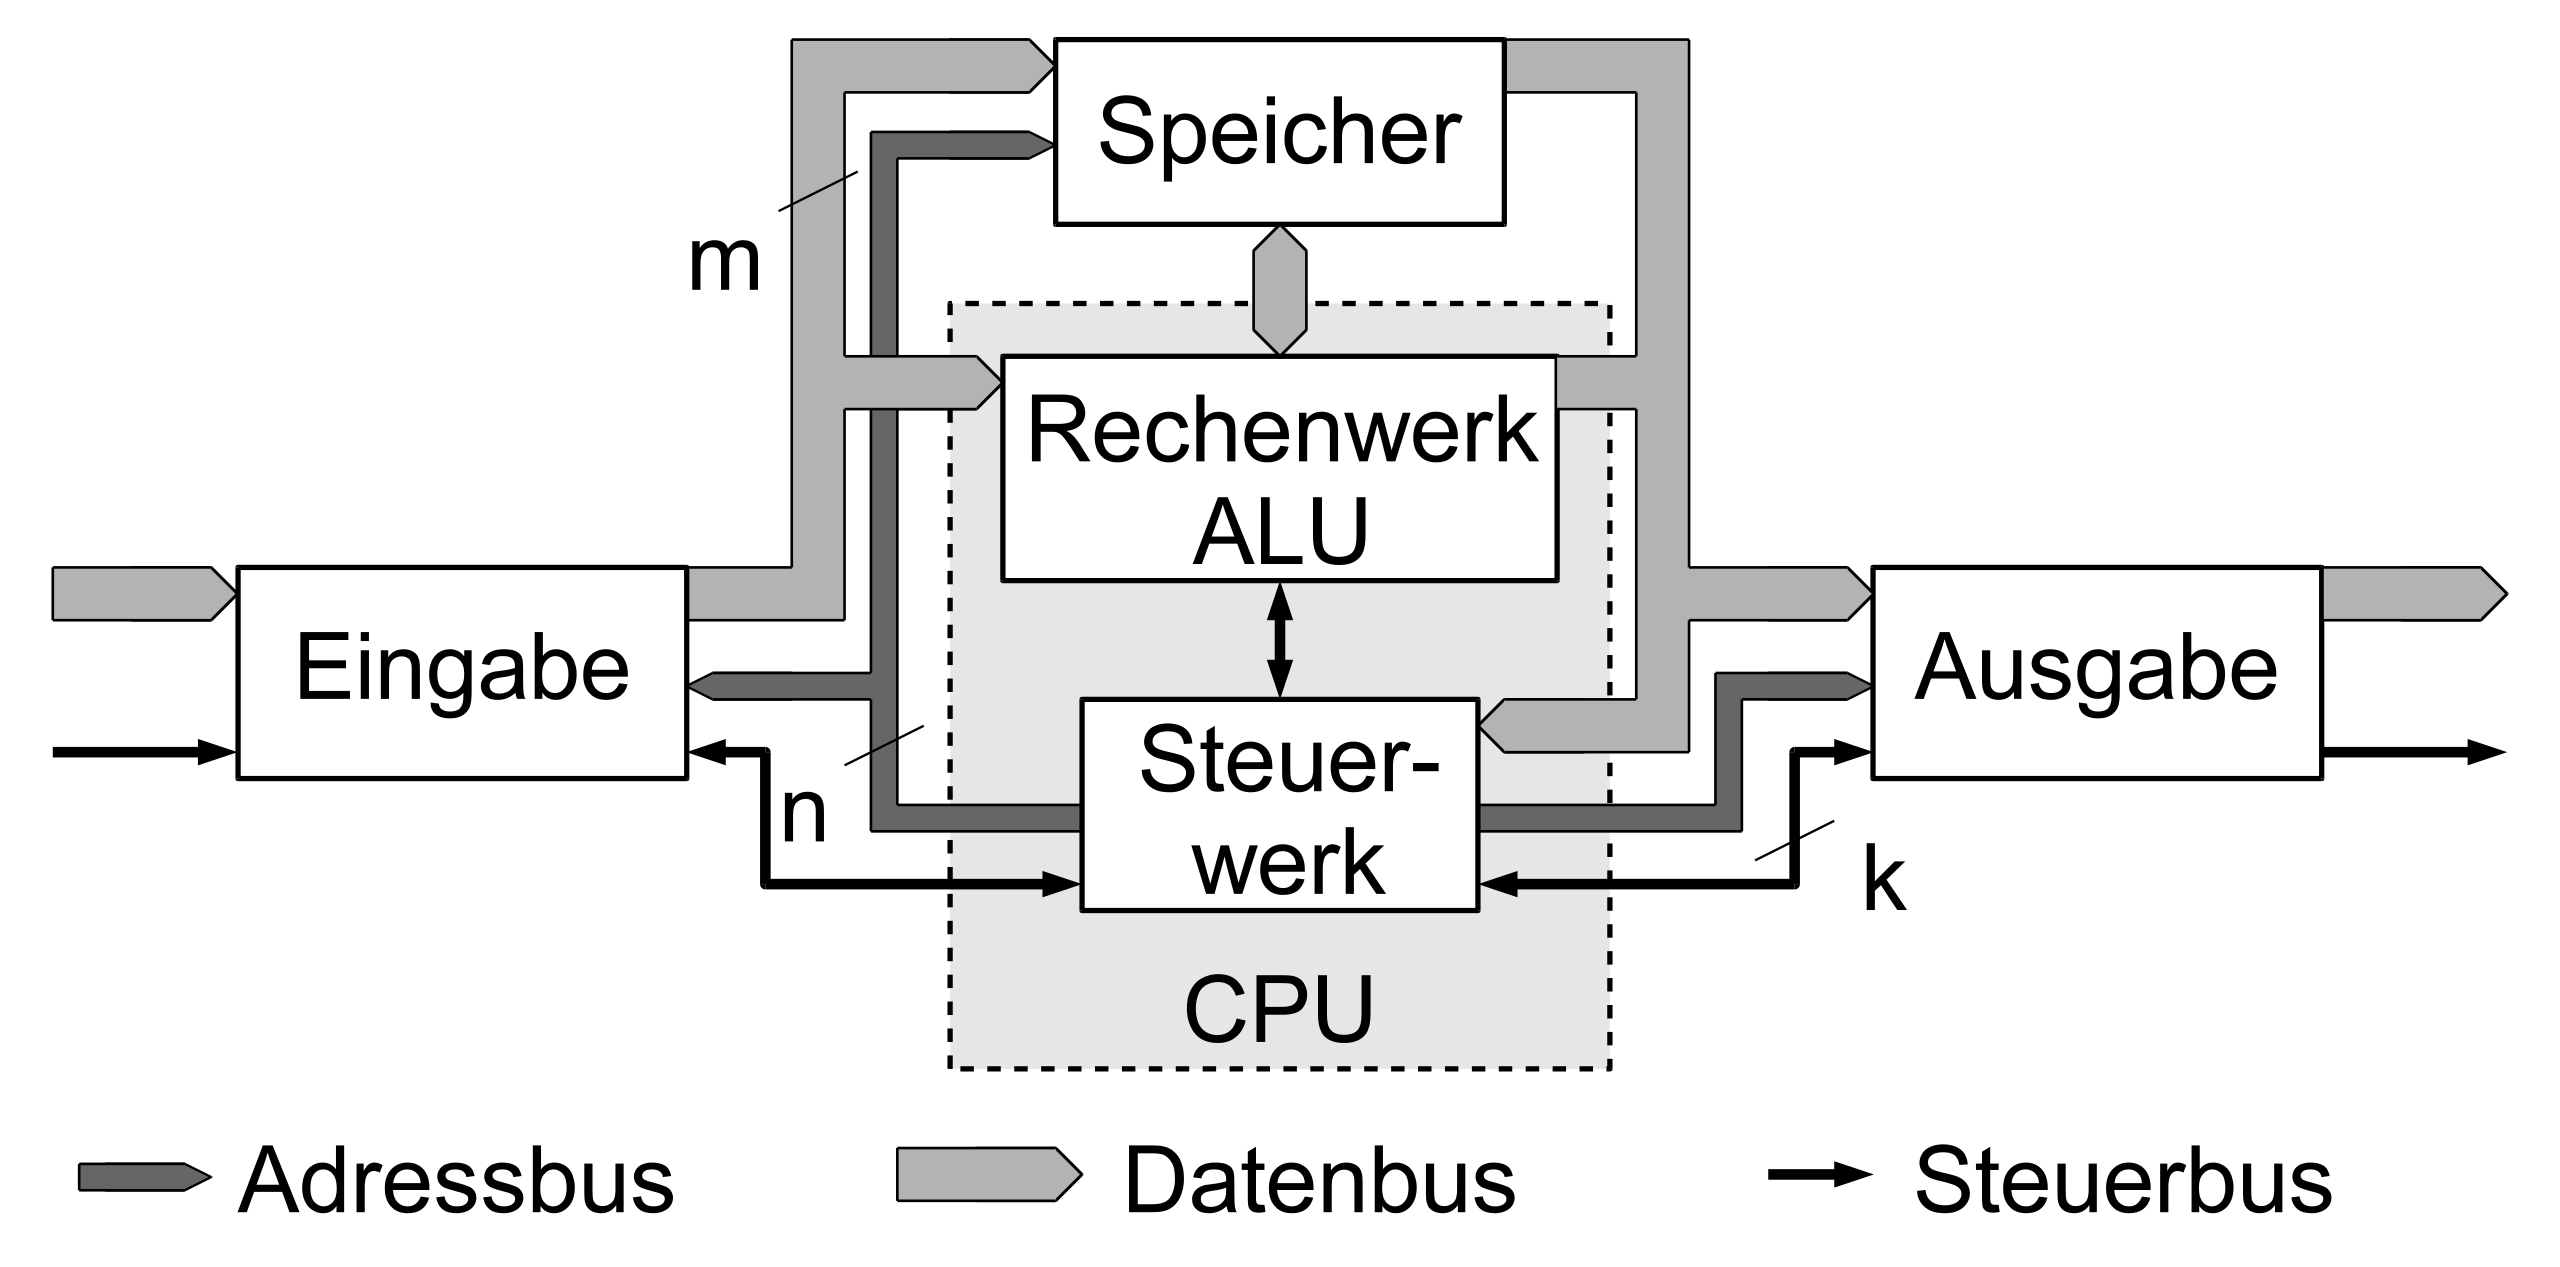
\includegraphics[width=0.8\textwidth]{Bilder/Von-Neumann-Architektur}
	\caption{Bildunterschrift}
	\label{fig:Bild} % Verweis mit \ref möglich
\end{figure}

\begin{itemize}

	\item CPU (Central Processing Unit)
	
	\begin{itemize}
		
		\item CU (Control Unit)
		
		\begin{itemize}
			\item Koordiniert die Ausführung von Befehle
		\end{itemize}
		
		\item ALU (Arithmetic Logical Unit) - \textcolor{red}{\textbf{Rechenwerk}}
		\begin{itemize}
			\item Das sind die Schaltkreise um die wirklichen Berechnung durchzuführen
		\end{itemize}
		
		\item Clock (Taktgeber)
		\begin{itemize}
			\item Sendet regelmäßig impulse aus, um einen Takt vorzugeben
			\item Ein Quwarz der mit Strom (CEmos Batterie) in Schwingung versetzt wird
		\end{itemize}
		
		\item PC ( Program counter - Programmzähler )
		\begin{itemize}
			\item Adressiert diejenige Zelle im Hauptspeicher (Memory) bei dem die nächste Anweisung beginnt
		\end{itemize}
	\end{itemize}
	
	\item Speicher (RAM)
	\begin{itemize}
		\item Speichert die Daten und Programme
		\item RAM (Random Access Memory)
		\begin{itemize}
			\item Speicher besteht aus Zellen
			\item Zellen sind durchnummeriert, z.B. von 0 bis n-1
			\item Alle Zellen sind gleich groß, zwischen 0 und x (Hardware abhängig)
			\item Jede Zelle speichert eine Zahl, repräsentiert in Bits
			\item 8 Bits/16 Bits/32 Bits/64 Bits - sind mögliche Variationen, jenachdem wie das System aufgebaut ist
		\end{itemize}
	\end{itemize}


	\item \textbf{Funktionalität} des Speichers: Lesen und Schreiben.
	\begin{itemize}
		\item Lese die Zelle 100 oder schreibe in die Zelle 100
		\item schreibe zahl z in Speicherzelle h
		\item wird in beliebiger Reihenfolge unterstützt
	\end{itemize}
	
	\item ROM (Read only Memory)
	
	\item Ein/Ausgabe (I/O)
	\begin{itemize}
		\item Sind Physikalische Geräte, die erlauben mit dem Computer von außerhalb zu Kommunizieren wie: Tastartur, Maus, Drucker, Kamera, Bildschirm, Netzwerkinterface, USB-Anschluss, ...usw.
	\end{itemize}
	
	\item BUS
	\begin{itemize}
		\item sind Kabel/Leitungen/Drähte, die alle Komponenten miteinander verbinden
	\end{itemize}
\end{itemize}

\subparagraph{\textbf{Funktionsweise}}
Solange der Rechner eingeschaltet ist, führt er die folgende Schritte immer wieder aus. \\
- FETCH - CU weißt den Memory über den Bus an, den Inhalt der Speicherzelle mit Adresse PC zu liefern \\
- DECODE - (Dekodiere/Interpretiere) CU schaut nach um welche Anweisung es sich handelt und holt gegebenenfalls weitere Bestandteile der Anweisung aus dem Memory \\
- EXECUTE - CU sorgt dafür, das Anweisung ausgeführt wird, indem sie die andere Komponente Koordiniert \\
- Aktualisiere PC \\
- REPEAT - Wiederholt den Durchlauf \\

\subsubsection{Programmiersprachen}

\subsubsection{Ausdrücke}

\subsubsection{Imperative Programmierung}

\subsection{Datentypen und Variablen}

\subsubsection{Primitive Datentypen}

\subsubsection{Zusammengesetzte Datentypen}

\subsubsection{Darstellung von Daten?}

\subsubsection{Die fünf Facetten von Variablen}

\subsection{Unterprogramme und Funktionen}

\subsubsection{Fundamentale Unterprogramme}

\subsubsection{Parameter Übergabe Strategien}

\subsubsection{Rekursion}

\subsubsection{Fünf schritte für die Implementierung von einer Funktion}

\subsubsection{Case Study ???}

\section{Algorithmen}
\subsection{Algorithmische Probleme}

\subsection{Sortieren}

\subsection{Laufzeit}

\subsection{Korrektheit}


\section{Funktionelle Programmierung}
\subsection{Funktionelle Programmierung in Scala}

\subsection{Listen und Hochrangige Funktionen}

\subsection{Dateitypen II}


\section{Objekt Orientierte Programmierung}
\subsection{Objekt Orientierte Programmierung}

\subsection{Queues and Stacks}

\subsection{Priority Queue}

\subsection{Dictionaries and Binary Search Trees}

\subsection{Begleitobjekte}
\begin{itemize}
	\item Teile globale Variablen zwischen Exemplaren einer Klasse.
\end{itemize}
\begin{minted}[frame=lines, linenos, fontsize=\small]{scala}
object Studi:
	private var mattrikel_zaehler: Int = 0

class Studi(var name: String, var fach: String):
	var mattrikel_nr = Studi.mattrikel_zaehler
	Studi.mattrikel_zaehler = Studi.mattrikel_zaehler + 1
	def getMat(): Int = mattrikel_nr

@main
def test(): Unit = 
	var s1: Studi = new Studi("Max", "Info")
	var s2: Studi = new Studi("Katharina", "Binfo")
	var s3: Studi = new Studi("Günther", "Winfo")
	println(s1.getMat())
	println(s2.getMat())
	println(s3.getMat())
\end{minted}

\subsection{Vererbung}
\begin{itemize}
\item Soll Ziele der Wiederverwendbarkeit \& Erweiterbarkeit unterstützen.
\item Können Beziehungen zwischen Klassen herstellen
\item Können neue Klassen zu \textbf{Unterklassen} von bestehenden Klassen machen!
\item \textbf{Unterklasse} übernimmt damit automatisch alle Methoden und Attribute der \textbf{Oberklasse}
\end{itemize}
\begin{minted}[frame=lines, linenos, fontsize=\small]{scala}
class Person(var name: String, private var age: Int):
	def mature(): Unit = 
		age = age + 1
	def getAge(): Int = age
	def work(): Unit = 
		println("werkel werkel")
\end{minted}

\begin{itemize}
	\item Inklusionspolymorphie:
	\begin{itemize}
		\item Objekte der Unterklasse sind typekompotibel mit der Oberklasse
	\end{itemize}
	\item Wir unterscheiden:
\begin{itemize}
	\item \textbf{Statischer} Typ einer Variable:
	\begin{itemize}
		\item Typ aus Variablendeklaration (ändert sich nicht - statisch)
		\item legt fest auf welche Attribute und Methoden zugegriffen werden kann
	\end{itemize}
	\item \textbf{Dynamischen} Typ einer Variable:
	\begin{itemize}
		\item Typ des Objekts, auf das die Variable aktuell verweist
	\end{itemize}
\end{itemize}
\end{itemize}
Wir können den statischen Typ einer Variable mit einem Cast(Typumwandlung - nur wenn der dynamische Typ es erlaubt) ändern(asInstanceOf). Wenn er es nicht erlaubt, sonst bekommen wir eine Class:CastException als Error von Scala.

\subsection{späte Bindung/Überschreiben}
\begin{minted}[frame=lines, linenos, fontsize=\small]{scala}
class Studi(name: String, private var age: Int, var fach: String) extends Person(name, age):
	def getZurMensa(): Unit = println("Mjam, schlürf")
	override def work(): Unit =
		println("studier studier")
		
var s1: Studi = new Studi("Max", 12, "Data Science")
var s1: Studi = Studi@6870f51a

scala> s1.work()
studier studier

var p1: Person = s1
var p1: Person = Studi@6870f52a

scala> p1.work()
studier studier

# zweite person
scala> var p2: Person = new Person("Moritz", 10)
var p2: Person = Person@1107891a

scala> p1 = p2
p1: Person = Person@234234a

scala> p1.work()
werkle werkle

# beispiel mit Array von Personen wird gezeigt...das schreibe ich jetzt nicht ab
scala> var ps: Array[Person] = Array(p2, s1)

for p <- ps do
	p.work()
	
#ausgabe von scala
werkel werkel
studier studier
\end{minted}

\begin{tcolorbox}[colback=blue!5!white, colframe=blue!75!black, title=Beispiel-Titel, width=\textwidth]
Dies ist eine farbige Textbox mit einem Titel, einem blauen Hintergrund und einem Rahmen.
\end{tcolorbox} %import OOP.tex teil


% Ausgabe meiner Quellen
\printbibliography

% Ende des Dokuments
\end{document}
